\chapter{Project Initialization}
\phantomsection


\setcounter{secnumdepth}{0} % Set the section counter to 0 so next section is not counted in toc

% ----------------------- Introduction ----------------------- %

\section{Introduction}
In this chapter, we are going to analyze the various specifications and requirements of the whole Aermax project from development to production.
We will also describe the product's main features.

\section{Overview of the Project}
The Aermax project is a comprehensive initiative aimed at developing a robust and scalable system through the integration of existing and newly developed microservices. This section provides an in-depth look at the architecture and key stakeholders involved in the project.

\subsection{Aermax Architecture}

The architecture diagram of Aermax shows the integration of existing and newly developed microservices within a unified virtual network environment.
\begin{itemize}
    \item \textbf{Existing Microservices}:
    \begin{itemize}
        \item \textbf{Operation Service}: Manages operations and interacts with the Operation Database .
        \item \textbf{User Service}: Handles user-related functionalities and interfaces with the User Database.
        \item \textbf{Keycloak Service}: Provides authentication and authorization services, connected to the Keycloak Database.
    \end{itemize}
    Our contributions to these existing microservices include adding new features, enhancements, and bug fixes.
    \item \textbf{New Microservices}:
    \begin{itemize}
        \item \textbf{Reward Service}: Manages reward-related processes and connects to the Reward Database. This service was developed from scratch.
        \item \textbf{Config Service}: A centralized microservice that interacts with all other microservices to provide configuration settings for the reward system. This service was also developed from scratch.
    \end{itemize}
\end{itemize}

This architecture supports modularity, scalability, and efficient management, ensuring consistent configurations and secure authentication through Keycloak.

\begin{minipage}{\linewidth}
    \centering
    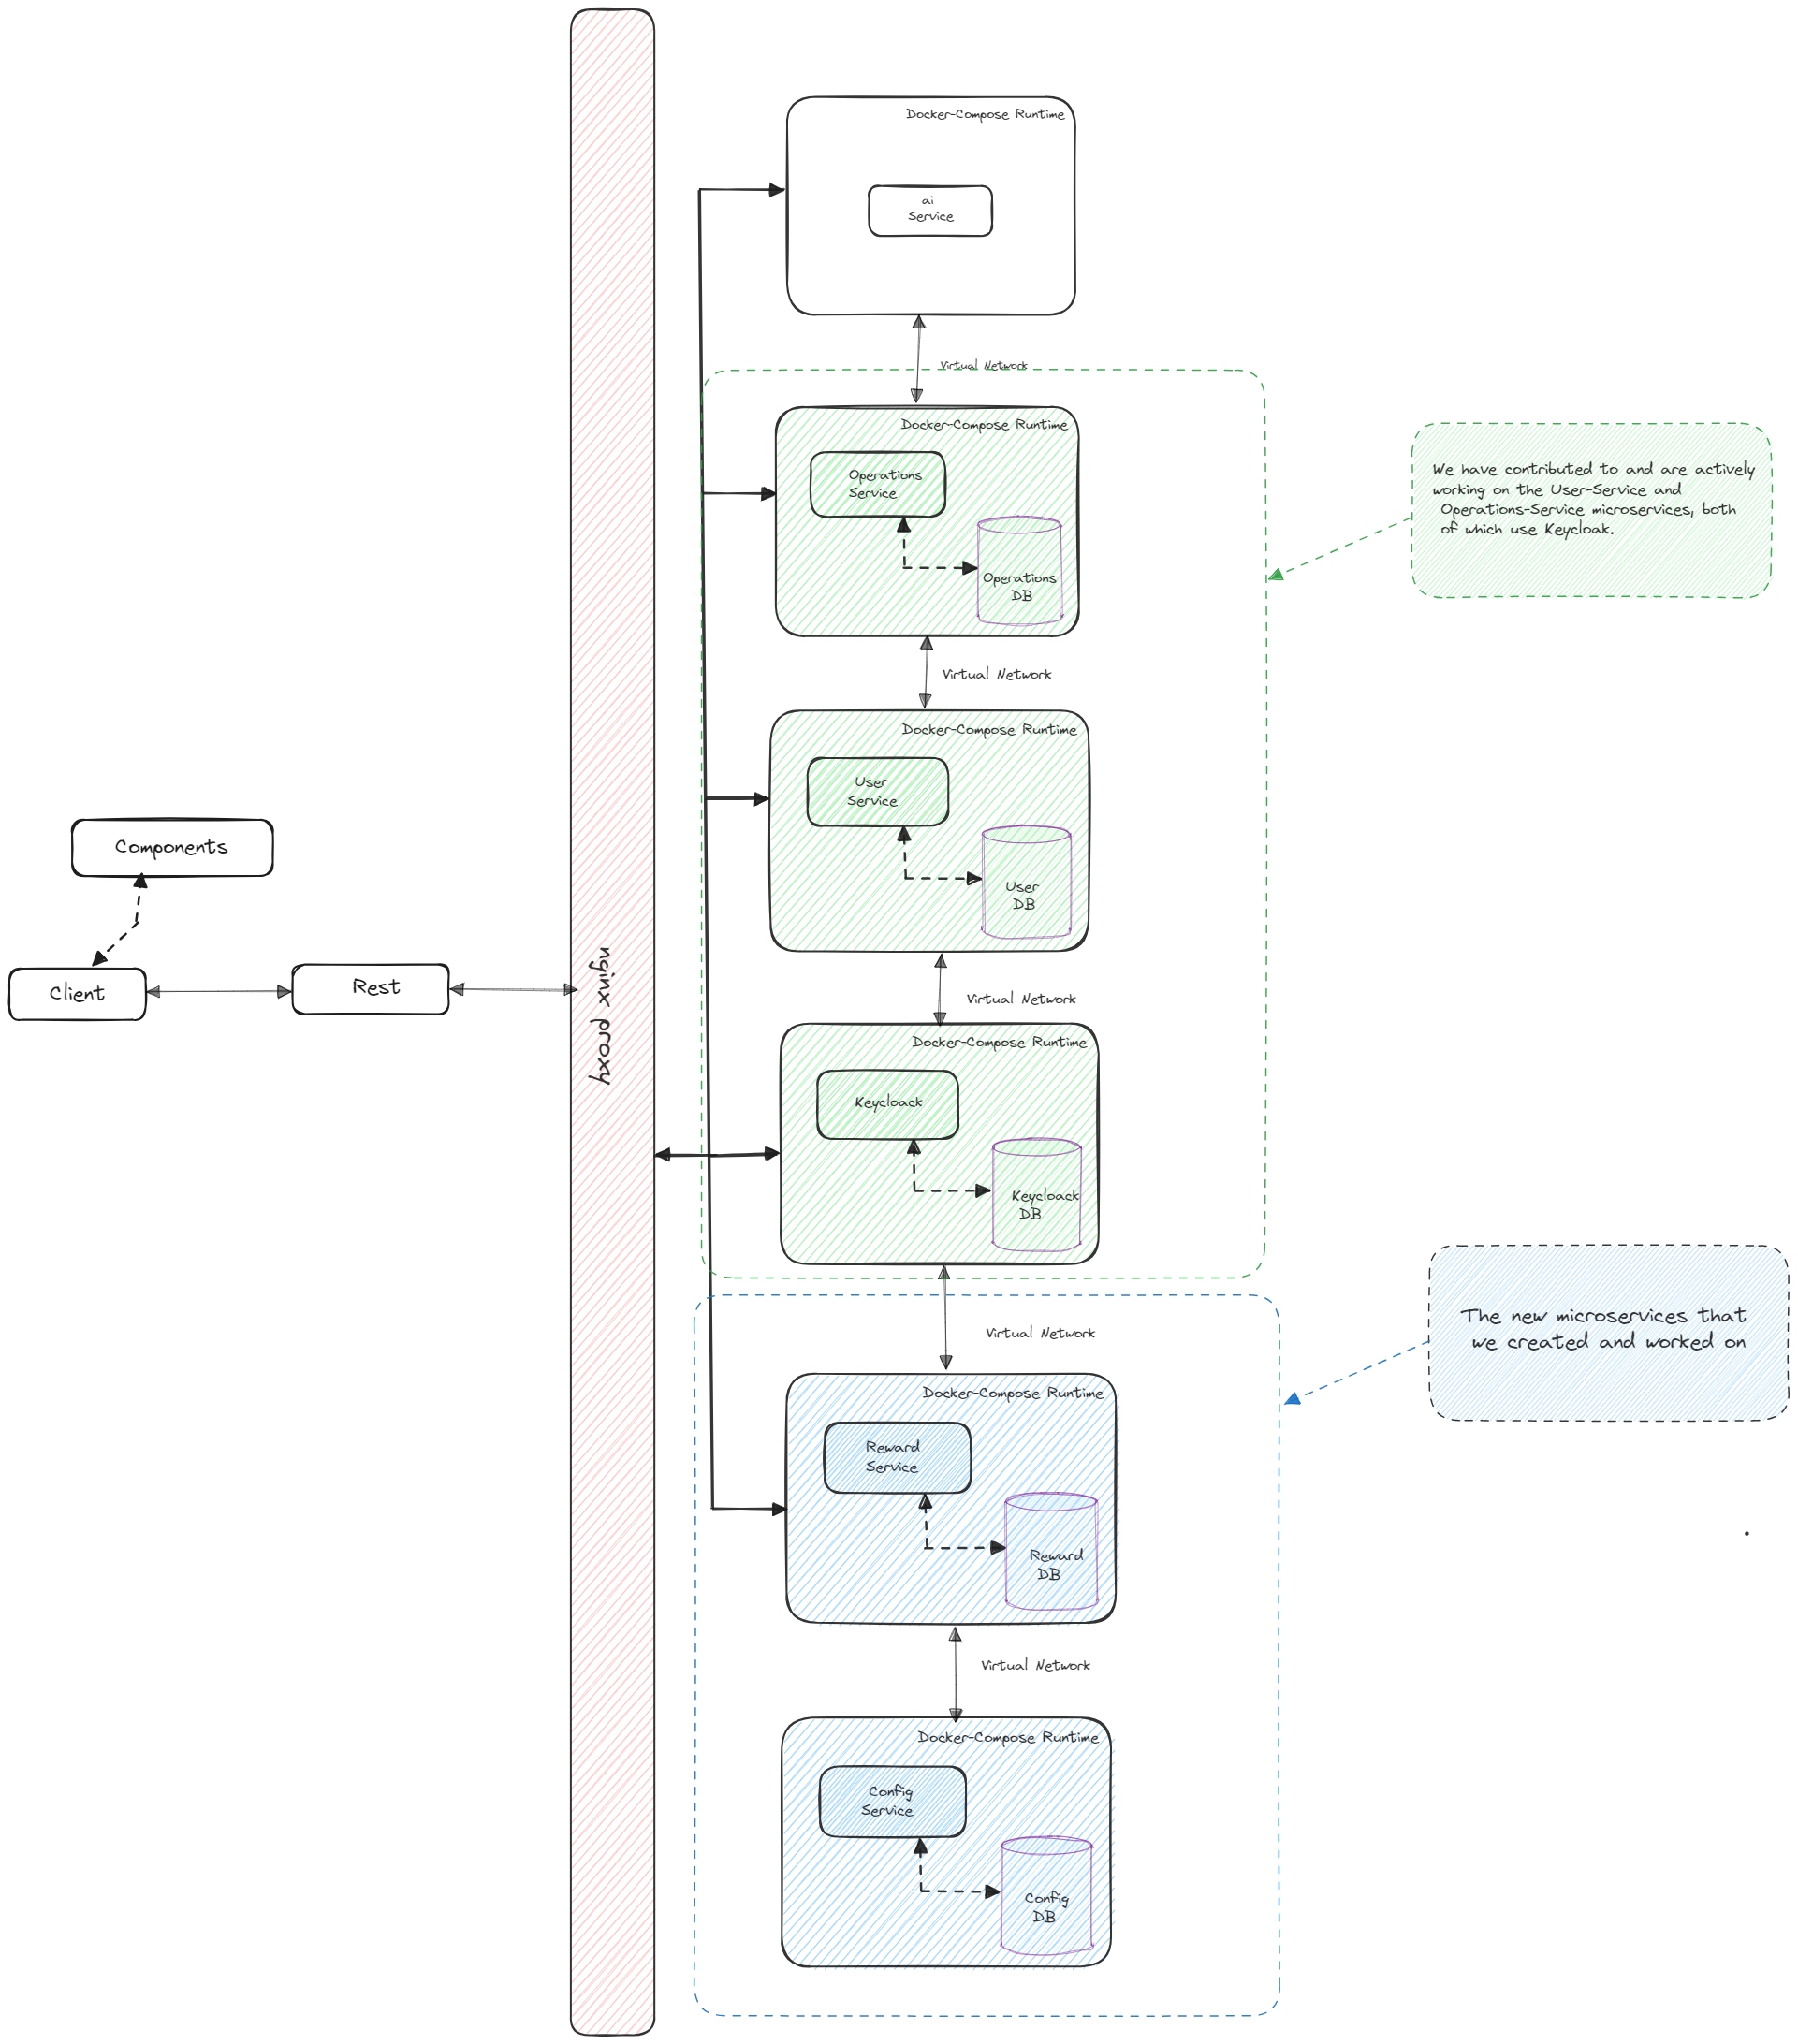
\includegraphics[width=15.5cm]{src/assets/chapters/AermaxArchitecture.png}
    \captionof{figure}{Aermax Architecture}
\end{minipage}

\subsection{Stakeholders}
The Aermax project involves various stakeholders who play crucial roles in its operation and success. The key stakeholders and their roles are summarized in the table below (Table \ref{tab:stakeholders_roles}). The grey-highlighted rows represent external stakeholders, while the non-highlighted rows represent internal stakeholders.

\begin{table}[h!]
    \centering
    \renewcommand{\arraystretch}{1.5} % Padding
    \caption{Stakeholders and their Roles}
    \label{tab:stakeholders_roles}
    \begin{tabularx}{\textwidth} {
            | >{\hsize=0.4\hsize\linewidth=\hsize\raggedright\arraybackslash}X
            | >{\hsize=1.6\hsize\linewidth=\hsize\raggedright\arraybackslash}X |}
        \hline
         \textbf{Role} & \textbf{Description} \\
        \hline
        Admin & Responsible for managing the overall system, including user management, system configuration, and monitoring. \\
        \hline
        \rowcolor{gray!20} Subcontractor & Industrial climbers who perform specific tasks or services outside the direct supervision of the project manager. \\
        \hline
        Employee & Internal staff members who work on various aspects of the project under the guidance of the project manager. \\
        \hline
        Project Manager & Oversees the project's progress, manages timelines, and ensures that all aspects of the project are aligned with strategic goals. \\
        \hline
        \rowcolor{gray!20} Leader & Provides vision and direction for the project, making high-level decisions and ensuring that the project aligns with organizational objectives. \\
        \hline
    \end{tabularx}
\end{table}
\section{Functional Requirements}
Functional requirements define the specific behaviors and functionalities that the system must possess to meet user needs. This section focuses on the key functional requirements for our project, particularly the reward system and other essential functionalities.

\subsection{Feature Enhancement}

This section details the latest upgrades and additions made to our system. These enhancements aim to improve functionality, usability, and overall user satisfaction. Key features introduced are:

\begin{itemize}
    \item \textbf{Dynamic Equipment List:} Implement a dynamic list of equipment that updates in real-time based on user selections and other criteria.
    \item \textbf{Bug Fixes:} Identify and fix several bugs in the existing functionalities to ensure a smooth user experience.
    \item \textbf{Enhanced Packet View:} Enhance the packet view by adding new functionalities and improving existing features.
    \item \textbf{Project Status Overhaul:} Overhaul the project status feature, including data migration to support the new structure.
    \item \textbf{Role System Overhaul:} Overhaul the role system to provide more granular control and better user management.
\end{itemize}

\subsection{Reward System}
The reward system is a crucial component of the application, designed to incentivize and engage users. The key functionalities of the reward system include:

\begin{itemize}
    \item \textbf{Points Accumulation:} Users earn points based on their activities and achievements within the application. The system must track and update points in real-time.
    \item \textbf{Points Redemption:} Users can redeem their accumulated points for various rewards. The system handles the redemption process, ensuring points are correctly deducted and rewards are delivered.
    \item \textbf{Reward Catalog:} A dynamic catalog of available rewards must be maintained, allowing users to browse and select rewards. The catalog should reflect current availability.
    \item \textbf{User Notifications:} The system should notify users about their points balance, reward availability, and updates related to the reward system.
\end{itemize}



\section{Technical Requirements}
Technical requirements specify the underlying technical aspects and constraints necessary for the system to function correctly. This section outlines the technical requirements that support the functional requirements.

\subsection{Data Management}
Proper data management is essential for the application's integrity and reliability. The system must provide the following technical functionalities:

\begin{itemize}
    \item \textbf{Database Integration:} The application should interact with multiple databases, such as 'reward-service-db' and 'config-service-db,' to store and retrieve data efficiently.
    \item \textbf{Data Synchronization:} Ensure data consistency and synchronization across different services and databases. Handle operations that span multiple microservices.
    \item \textbf{Data Security:} Implement robust security measures to protect sensitive user data, including encryption, access control, and regular security audits.
    \item \textbf{Backup and Recovery:} Support regular data backups and provide mechanisms for data recovery in case of failures or data loss.
\end{itemize}

\subsection{System Integration}
Seamless integration with various external and internal systems is crucial for the application's operation. Key technical integration functionalities include:

\begin{itemize}
    \item \textbf{RabbitMQ Configuration:} Retrieve and manage RabbitMQ configurations from the config service for different microservices. Ensure reliable message queuing and processing.
    \item \textbf{Health Checks:} Implement health checks for various microservices to monitor their status and ensure they are operating correctly.
    \item \textbf{Deployment Pipeline:} Set up a deployment pipeline for staging and production environments, including automated testing, deployment, and monitoring of the reward system.
\end{itemize}

% --------------- Non-functional Requirements --------------- %

\section{Non-functional Requirements}
Non-functional requirements describe any specification that does not add direct business value but is nonetheless crucial for the good operation of developed software.
For Aermax, what we should focus on is:
\begin{itemize}
	\item \textbf{Reliability and Availability:} The software should be available 24 hours a day and 7 days a week.
	\item \textbf{Security:} Clients should be able to safely log in to the dashboard with a strong authentication system.
	\item \textbf{Scalability:} This is the main reason we're using new microservices.
	\item \textbf{Documentation:} We should always document each and every step we make extensively so that new developers can onboard on the project in a fast and efficient way, which further emphasizes reliability.
\end{itemize}

\section{Technologies}
A project can always look simple from the outside, however if we dive deeply into how most software is made, we can see that it's not that simple of a process.
Therefore, this part will list all of the technologies that we've used and also some of the major technical difficulties we've encountered during the realization of our project.

\medskip

\begin{itemize}
    \item \textbf{Kubernetes:} \newline The most powerful tool for managing containerized workloads in the cloud. \newline
          \begin{minipage}{\linewidth}
              \centering
              
\includegraphics[width=3cm]{src/assets/logos/kubernetes_512x512.png}
              \captionof{figure}{Logo of Kubernetes}
          \end{minipage}
    \item \textbf{LaTeX:} \newline \cite{latex-project} A high-quality document preparation and typesetting system for technical grade documents. \newline \newline
          \begin{minipage}{\linewidth}
              \centering
              
\includegraphics[width=3cm]{src/assets/logos/latex_200x200.png}
              \captionof{figure}{Logo of The LaTeX Project}
          \end{minipage}
    \item \textbf{Spring Boot:} \newline A powerful framework for building Java-based enterprise applications

. \newline \newline
          \begin{minipage}{\linewidth}
              \centering
              
\includegraphics[width=6.5cm]{src/assets/logos/Springboot.png}
              \captionof{figure}{Logo of Spring Boot}
          \end{minipage}
    \item \textbf{ReactJS:} \newline A JavaScript library for building user interfaces. \newline \newline
          \begin{minipage}{\linewidth}
              \centering
              
\includegraphics[width=3.5cm]{src/assets/logos/reactjs.png}
              \captionof{figure}{Logo of ReactJS}
          \end{minipage}
    \item \textbf{Keycloak:} \newline An open-source identity and access management solution. \newline \newline
          \begin{minipage}{\linewidth}
              \centering
              
\includegraphics[width=6.5cm]{src/assets/logos/Keycloak-logo.png}
              \captionof{figure}{Logo of Keycloak}
          \end{minipage}
    \item \textbf{Python:} \newline A versatile programming language used for various types of software development. \newline \newline
          \begin{minipage}{\linewidth}
              \centering
              
\includegraphics[width=6.5cm]{src/assets/logos/python.png}
              \captionof{figure}{Logo of Python}
          \end{minipage}
    \item \textbf{NestJS:} \newline A framework for building efficient, reliable, and scalable server-side applications. \newline \newline
          \begin{minipage}{\linewidth}
              \centering
              
\includegraphics[width=6.5cm]{src/assets/logos/nestjs_logo_icon.png}
              \captionof{figure}{Logo of NestJS}
          \end{minipage}
    \item \textbf{React Query:} \newline A library for fetching, caching, and synchronizing server state in React applications. \newline \newline
          \begin{minipage}{\linewidth}
              \centering
              
\includegraphics[width=5.5cm]{src/assets/logos/react-query.png}
              \captionof{figure}{Logo of React Query}
          \end{minipage}
    \item \textbf{Langchain:} \newline A framework for developing applications powered by language models. \newline \newline
          \begin{minipage}{\linewidth}
              \centering
              \includegraphics[width=6.5cm]{src/assets/logos/langchain.png}
              \captionof{figure}{Logo of Langchain}
          \end{minipage}
\end{itemize}

\section{The Application’s Microservices}
\textbf{Table 9: All the Application’s Microservices}
\begin{longtable}{|p{3cm}|p{7cm}|p{2cm}|}
    \hline
    \textbf{Name} & \textbf{Description} & \textbf{Scalable} \\
    \hline
    \endhead
    ai-service & Manages AI operations, including data processing and ML algorithms. & Yes \\
    \hline
    user-service & Handles user data, security, and support functions. & Yes \\
    \hline
    operations-service & Coordinates project management and operational workflows. & Yes \\
    \hline
    storage-service & Oversees data storage and database management. & Yes \\
    \hline
    client & Provides the user interface and input processing. & Yes \\
    \hline
    reward-service & Manages the reward system, including points accumulation, redemption, and catalog maintenance. & Yes \\
    \hline
    config-service & Stores and retrieves configuration settings for various services. & Yes \\
    \hline
    topix-service & Manages SOAP-based communications and topics. & Yes \\
    \hline
\end{longtable}

\section{Conclusion}
Defining and implementing these functional and technical requirements is crucial for developing a robust, reliable, and user-friendly Aermax application that meets the needs of our users and stakeholders, ensuring scalability, security, and comprehensive functionality.